\documentclass[a4paper]{article}
 
\usepackage{amsmath}
\usepackage{graphicx}
\usepackage{caption}
\usepackage{subfigure}
\usepackage{epstopdf}
\usepackage[ansinew]{inputenc}
\usepackage{listings}
\usepackage{xcolor}
%\setlength{\oddsidemargin}{0cm}
%\setlength{\evensidemargin}{0cm}
%\setlength{\topmargin}{0cm}

\usepackage[]{algorithm2e}

\usepackage{a4wide}

\title{ Allen mouse brain circuit - visual debugging }
%\author{Till Schumann}
%\date{}

\begin{document}
   \maketitle
   
   \section{Description}
   A simulation of a full scale point neuron circuit of the mouse brain make great demands on the simulator, circuit generation and the used data formats.
   The full point neuron circuit contains $75e6$ neurons with around $1e4$ synapses per neuron.     
   Allen Institute for Brain Science provides a high-resolution map of neural connections in the mouse brain.
   It contains several injection experiments. The provided datasets of the experiments 
   contain a 3D image of the injection and a 3D image of its axonal projection labeled by viral
   tracers. Based on this data the long range connections for the point neuron circuit of the mouse brain are generated.   
   
   \section{Given data}
   Besides x,y,z coordinate of each neuron and the synapse information (source and target neuron id), the 3d injection and projection images are given.
   Further a 3d picture which contains the number of excitatory neurons per pixel is given. From this a 3d model of mouse brain can be generated.  
   
   \begin{figure}[ht!]
   	\begin{center}
        \subfigure[Injection sites - showing all available experiments]{%
            \label{fig:allInjections}
            \includegraphics[width=0.4\textwidth]{../connectionBrowser_allinjections.png}
        }
        \hspace{1cm}
        \subfigure[Projection of one experiment]{%
            \label{fig:oneProjection}
            \includegraphics[width=0.32\textwidth]{../connectionBrowser_oneinjections.png}
       }
    	   \end{center}
    	\caption{%
        The pictures are inverted and copied from the Allen Brain Atlas.
     }%
   \label{fig:atlas}
   \end{figure}
   
   \begin{figure}[ht!]
   	\begin{center}
        \subfigure[Number of excitatory neurons per voxel]{%
            \label{fig:allInjections}
            \includegraphics[width=0.4\textwidth]{../exNeurons_numPerVoxel.png}
        }
        \hspace{1cm}
        \subfigure[Illustration of neurons inside an injection and projection area]{%
            \label{fig:oneProjection}
            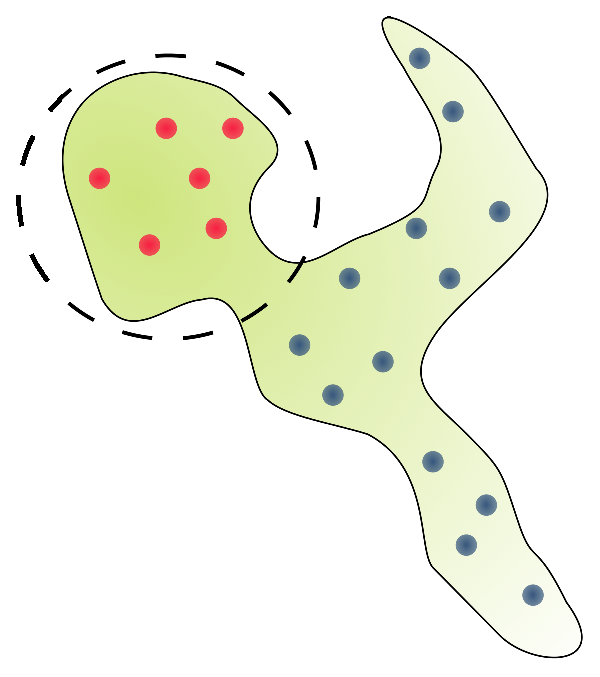
\includegraphics[width=0.35\textwidth]{drawing.eps}
       }
    	   \end{center}
    	\caption{%
        The plots (x vertical and z horizontal axis) show a slice (along the y axis) of the 3D datasets. 
     }%
   \label{fig:atlas}
   \end{figure}
   \newpage
	
	
	

\end{document}
